\documentclass{beamer}

\usepackage{amsmath,amsfonts}
\usepackage[math]{fontspec}
\usepackage{fontenc}
\setmainfont{Droid Serif}

\mode<presentation>
{
%\usetheme{PaloAlto}
%\useoutertheme{tree}
\usecolortheme{lily}
\useinnertheme{rectangles}
\setbeamercovered{transparent}
\setbeamertemplate{blocks}[rounded][shadow=true]
}

\begin{document}

\begin{frame}
  Les slides sont disponibles sur
  \begin{center}
    \centerline{\url{https://github.com/cemosis/unistra.ufr.math}}
  \end{center}
\end{frame}

\section{Analyse Fonctionnelle Avancée et Applications aux EDP}

\begin{frame}\frametitle{Analyse Fonctionnelle Avancée et  EDP}
  \begin{block}{Objectifs}
    \begin{itemize}
    \item Préparation du M2MF 2015-2016
    \item Acquisition du vocabulaire et des outils mathématiques nécessaires à
      l'analyse des équations aux dérivées partielles
    \end{itemize}
  \end{block}
  \begin{block}{Objets}
    Étant donné $\Omega \subset \mathbb{R}^d, d=1,2,3$, les espaces $H^s(\Omega)$
    \begin{equation*}
      H^s(\Omega)=\{ u \in L^2(\Omega)~|~\forall\alpha\text{ tel que }|\alpha|\le s,~D^\alpha u\in L^2(\Omega)\}
    \end{equation*}
  \end{block}
  \begin{block}{Questions}
    \begin{itemize}
    \item Propriétés de ces espaces
    \item Applications aux EDP: cadre fonctionel pour montrer
      l'existence et unicité de solutions
    \end{itemize}
  \end{block}
\end{frame}

\begin{frame}\frametitle{Analyse Fonctionnelle Avancée et EDP}

  \begin{block}{Quelques exemples d'EDP: probl\`emes d'\'evolution}

Evolution d'une solution en temps $t$ sur un domaine $\Omega$. La solution est donn\'ee implicitement par une \'equation, des conditions limites (au bord du domaine)
et une donn\'ee initiale. Formalisation sous la forme
$$
\frac{d u}{dt}+Au = 0,\ u(0) = u_0
$$

{\bf Equation de la chaleur:} mod\'elise la distribution de temp\'erature $u$ dans un domaine $\Omega$ \`a l'instant $t$

$$
\partial_t u -\Delta u = 0
$$

{\bf Equation des ondes:} mod\'elise %les petites vibrations d'une corde (en dimension $1$) ou d'une membrane \'elastique (en dimension $2$), ou plus g\'en\'eralement
la propagation d'une onde (acoustique, \'electromagn\'etique...)

$$
\partial_t^2u-\Delta u = 0
$$

R\'ef\'erence: Ha\"im Brezis, Analyse Fonctionnelle

  \end{block}


\end{frame}


\section{Méthodes Numériques pour les EDP}

\begin{frame}{Méthodes Numériques pour les EDP}


  \begin{columns}
    \column{.5\linewidth}
    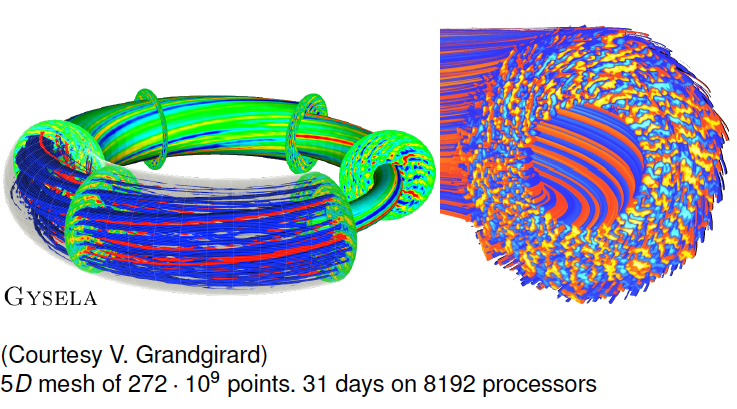
\includegraphics[width=0.9\linewidth]{gysela.png}\\
    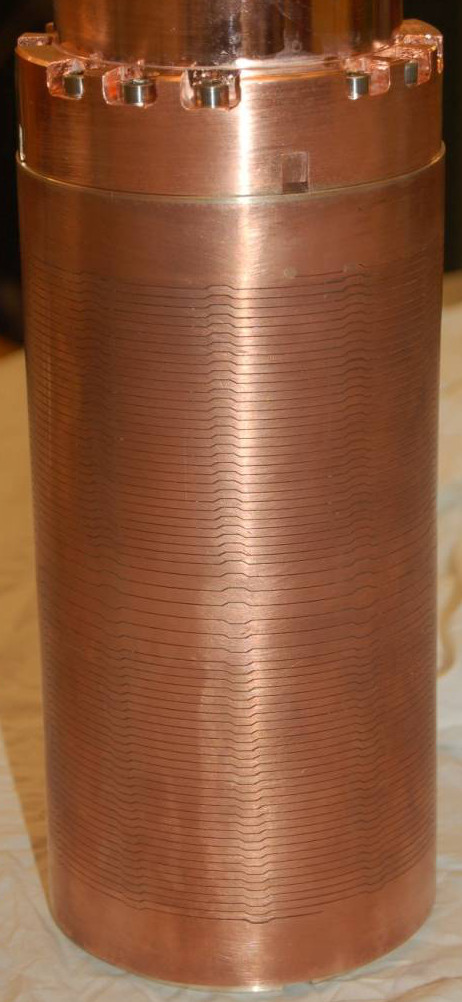
\includegraphics[width=0.4\linewidth]{Radial_magnet.jpg}
    \includegraphics[width=0.4\linewidth]{temperature.jpg}
    \column{.5\linewidth}
    \centerline{\includegraphics[width=9\linewidth]{MesoChallengePressure2.png}}\\
  \end{columns}




\end{frame}
\begin{frame}{Méthodes Numériques pour les EDP: Rao \& Prud'homme}
  \begin{block}{Objectifs}
    \begin{itemize}
    \item Étude mathématique et numérique de la méthode des éléments
      finis qui propose un cadre général pour passer de formulations
      continues à discrètes
    \item le cadre théorique est donnée par le cours d'Analyse
      Fonctionnelle Avancée
    \end{itemize}
  \end{block}
  \begin{block}{Questions}
    \begin{itemize}
    \item Existence et unicité de solution pour des problèmes
      elliptiques linéaires coercifs au niveaux continus et discrets
    \item Construction de fonctions de bases, dites élément fini
    \item Erreur d'interpolation et d'approximation en norme $L^2$ et $H^1$
    \item Implémentation de la méthode et Vérification numériques des théorèmes
    \end{itemize}
  \end{block}
\end{frame}

\begin{frame}{Vers le M2}

  \begin{block}{M2R Analyse 2015-2016}
    \begin{itemize}
    \item Systèmes hyperboliques (B. Rao, P. Helluy)
    \item Réductions de modèles.
      \begin{itemize}
      \item Méthode des bases réduites (C. Prud'homme)
      \item Méthode d'homogénéisation (S. Hirstoaga)
      \end{itemize}
    \item Théorie et approximation des EDP paraboliques
      \begin{itemize}
      \item Théorie et approximation (Z. Belhachmi)
      \item Application à l'interaction
        fluide-structure (C. Murea)
      \end{itemize}
    \end{itemize}
  \end{block}

\end{frame}
\end{document}
